\section{Einleitung}

In dieser Ausarbeitung geht es um die Lösung eines konkreten
\emph{Travelling Salesman Problems} (TSP).

\begin{quote}
Das Problem des Handlungsreisenden (auch Rundreiseproblem, engl.
Traveling Salesman Problem oder Traveling Salesperson Problem (TSP))
ist ein kombinatorisches Optimierungsproblem des Operations Research und
der theoretischen Informatik. Die Aufgabe besteht darin, eine Reihenfolge
für den Besuch mehrerer Orte so zu wählen, dass die gesamte Reisestrecke
des Handlungsreisenden nach der Rückkehr zum Ausgangsort möglichst
kurz ist. \citep{wikiTsp}
\end{quote}

\noindent Da dieses Problem NP-vollständig ist, lässt es sich nur mit
exponentiellem Zeitaufwand lösen.
Dies ist für kleine Mengen an Orten noch machbar, aber für eine große
Menge an Orten wird der Zeitrahmen schnell gesprengt.
Beispiel:

\begin{itemize}
  \item 5 Orte entsprechen $5! = 120$ mögliche Reisestrecken.
  \item 29 Orte entsprechen $29! \approx 9 \cdot 10^{30}$ mögliche Reisestrecken.
\end{itemize}

\noindent Bei einem Rechner, der $10^{5}$ Berechnungen der Reisestreckenlänge pro
Sekunde schafft, bedeutet das im Fall von fünf Orten eine Rechenzeit
von ca. 1 ms (einer Millisekunde) um herausgefunden, welche die kürzeste Strecke ist.
Bei 29 Städten bräuchte dieser Rechner ca. $9 \cdot 10^{16}$
Jahre\footnote{Das Universum ist
knapp $13,7 \cdot 10^{9}$ Jahre alt. \citep[siehe][]{wikiUniversum}}!
Das macht es quasi unmöglich das TSP Problem mit einer naiven Implementierung
in angemessener Rechenzeit zu lösen.
Mit Hilfe heuristischer Optimierungsverfahren kann dieses Problem
jedoch troztdem in angemessener Zeit gelöst werden. Hier eine Definition
von \citep{fink}:

\begin{quote}
Heuristische Optimierungsverfahren sind universell einsetzbare Verfahren,
welche mit realitätsverträglichem Rechenaufwand hochwertige Lösungen
ermitteln und damit zur effektiven Bewältigung realer Entscheidungsprobleme
beitragen können. \citep[S.~1]{fink}
\end{quote}

\begin{quote}
Ausgehend von einem entwickelten wohlstrukturierten Problemmodell sind 
Optimierungsverfahren erforderlich, welche die Auswahl aus der Menge der 
Handlungsalternativen (im Sinne von möglichen Lösungen/Plänen) automatisch
vornehmen oder unterstützen. \citep[S.~3]{fink}
\end{quote}

\begin{quote}
Heuristiken sind auf Erfahrung [...] beruhende Vorgehensweisen zur
Suche nach guten, aber nicht notwendigerweise optimalen Lösungen
[...] für bestimmte Planungsprobleme. \citep[S.~4]{fink}
\end{quote}

\paragraph{Dokument} Dieses Dokument
ist während des Wintersemesters 2013/2014 als das
Ergebnis der Aufgabenstellung aus der Vorlesung
\emph{Heuristische Optimierungsverfahren} entstanden.
Die Aufgabe bestand darin „einen evolutionären Algorithmus zur Lösung von
Travelling Salesman Problems (TSP)“ mit der Softwarebibliothek GEATbx zu entwickeln.
Der Hauptteil besteht darin „einige der [...] Parameterwerte und Optionen“ zu
modifizieren „und die Auswirkungen solcher Änderungen auf die Güte des Algorithmus“
zu untersuchen.
Dabei ist das Ziel den Algorithmus so zu konfigurieren, dass er
„möglichst gute Lösungen in möglichst kurzer Zeit ermittelt.“ \citep[Aus][]{aufg}

Genetische bzw. evolutionäre Algorithmen wurden maßgeblich von den Teams
John von Holland, K. A. De Jong (Universität Michigan) und
Ingo Rechenberg, Hans P. Schwefel (TU Berlin) unabhängig voneinander erdacht.
\citep[Vgl.][]{erben}

\begin{quote}
[Die] gemeinsame[n] Grundlagen [von evolutionären Algorithmen] liegen in der
Kodierung möglicher Lösungen als Zeichenketten und der primären Anwendung von
Rekombinationsoperatoren auf eine Menge (Population) von möglichen Lösungen
(Individuen). Derartige Verfahren imitieren damit die Prinzipien der
natürlichen Evolution, bei der die Eigenschaften eines Individuums durch
Chromosome kodiert werden, mit Hilfe von Rekombinationsoperatoren neue
Individuen erzeugt werden und das Überleben bzw. Fortpflanzen von Individuen
durch Selektionsprozesse in Abhängigkeit von deren
„Fitness“ gesteuert wird. \citep[S.~6]{fink}
\end{quote}

\noindent Das Dokument ist vom Aufbau her der Aufgabenstellung nachempfunden.
Zunächst wird das Datenformat der Datei in der die Orte definiert sind
beschrieben, darauf folgen einige Testläufe und deren Ergebnisse mit
den voreingestellten Parametern.
Im Kapitel \ref{sec.param} werden die möglichen Parameter und ihre
Auswirkungen beschrieben.
Um die bestmöglichen Parameter herauszufinden, wurde ein automatisiertes
Testsystem geschaffen. Der Aufbau des Testsystems wird in Kapitel
\ref{testsystem} genauer beschrieben.
In den Kapiteln \ref{populations} bis \ref{mutation} werden die Ergebnisse
präsentiert und diskutiert, darauf folgt eine Zusammenfassung in der
die idealen Parameter zusammengeführt werden, um das finale und
ideale Ergebnis zu finden.

Die Auswertung der Ergebnisse wurde mit Hilfe von einigen selbstgeschriebenen
Python-Skripten soweit automatisiert, dass ein beträchtlicher Teil des
Dokuments gänzlich automatisch und konsistent generiert werden kann.
Sämtliche Tabellen sowie die zugehörigen Diagramme sind auf diese Art
generiert worden.
Das bedeutet, wenn der Auswertungsserver neue Resultate an das
Repositorium übergibt, werden diese beim nächsten Bauen des PDFs
direkt als ausgewertete Tabelle mit Diagramm dargestellt.
Sämtlicher MATLAB- (Simulation), Python- (Auswertung) und LaTeX-Code (Dokument)
ist im Git-Repositorium \emph{HeurOptAusarbeitung}\footnote{
GitHub Link: \url{https://github.com/themerius/HeurOptAusarbeitung}} auf GitHub
zu finden. 


\section{Vorbereitungen}


\subsection{Datenformat}

\noindent In der Datei {\tt bays29.tsp} sind 29 bayrische Städte aufgeführt.
Der Kern der Datei ist die 29x29 Matrix, welche die Reisekosten zwischen
den einzelnen Städten beschreibt. Dieser Städte-Graph ist zur Lösung
des Travelling-Salesman-Problems (TSP) gedacht.
Details des Aufbaus der Datei:

\begin{itemize}
  \item Header.\\
  Name, Problemtyp, Kommentar, Dimension des Problems bzw. der Matrix, Typ und Format der Kantengewichte
  \item Kantengewichte.\\
  29 x 29 Matrix mit den Reisekosten zwischen den einzelnen Städten als symmetrische Matrix, d.h. es handelt sich um einen ungerichteten Graphen.
  \item Positionen der Städte.\\
  Liste mit Stadtnummer und X-, Y-Koordinaten, welche die Städtepositionen beschreiben.
  Diese Informationen sind lediglich zur Visualisierung (MATLAB Plot) nötig.
\end{itemize}


\subsection{Testläufe mit tspVorlage.m}

Das {\tt tspVorlage.m} Skript wurde 15 mal ausgeführt, die Ergebnisse in
Tabelle \ref{testlaeufe} festgehalten und auf Abbildung \ref{fig.testlaeufe}
visualisiert.
Eine kleine Auswertung ergibt einen Mittelwert von 3077.93 km mit
einer Standardabweichung von 177.05 km.
Das Minimum beträgt 2764 km und das Maximum 3490 km.

Laut \cite{aufg} liegt die beste
Lösung\footnote{In der Software \emph{best objective value} genannt.},
also der kürzeste Weg für eine Rundreise, bei 2020 km.
Das bedeutet, hier gibt es noch Optimierungsbedarf.
In den Kapiteln \ref{populations} bis \ref{mutation} werden systematisch bessere Einstellungsparameter
gesucht, um einen möglichst kurzen Weg mit möglichst geringer Laufzeit zu finden.

\begin{table}[h]
\begin{tabular}{ | r | c | c | }
  \hline
  \# Iteration & kürzester Weg & in Generation \\
  \hline
  1  & 3324 & 288 \\
  2  & 3041 & 345 \\
  3  & 3180 & 388 \\
  4  & 3148 & 244 \\
  5  & 3102 & 372 \\
  6  & 2898 & 243 \\
  7  & 2980 & 287 \\
  8  & 2764 & 139 \\
  9  & 2982 & 307 \\
  10 & 3490 & 319 \\
  11 & 2974 & 293 \\
  12 & 3281 & 364 \\
  13 & 2991 & 313 \\
  14 & 2967 & 261 \\
  15 & 3047 & 353 \\
  \hline
\end{tabular}
\caption{Testläufe mit {\tt tspVorlage.m}}\label{testlaeufe}
\end{table}

\begin{figure}[h!]
  \centering
  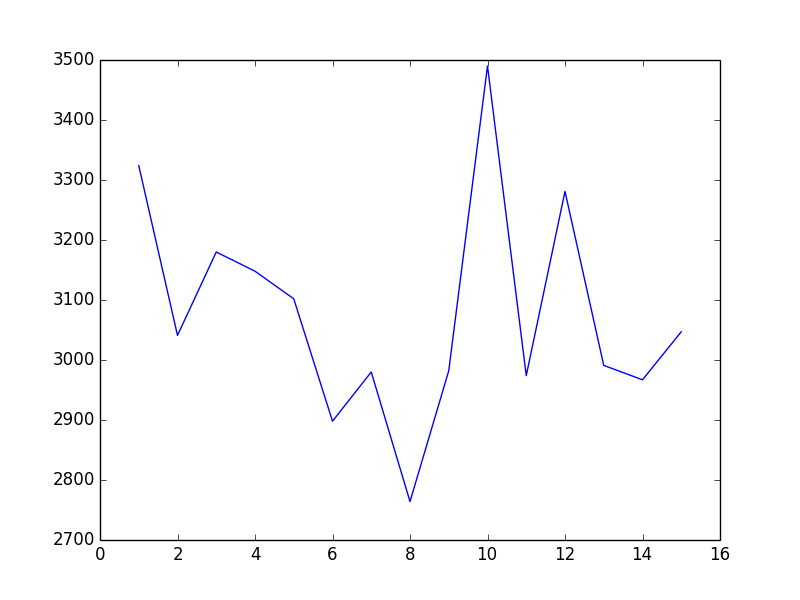
\includegraphics[width=1.0\textwidth]{Figures/gen/tspVorlage.png}
  \caption{Testläufe mit {\tt tspVorlage.m}}\label{fig.testlaeufe}
\end{figure}


\subsection{Parameter und Optionen}\label{sec.param}

Mit der Methode {\tt geaoptset( Key, Value )} können beliebig viele
Parameter an den evolutionären Algorithmus übergeben\footnote{Natürlich
muss der Algorithmus diese Parameter auch verarbeiten können.} werden.
Eine nochmalige Zuweisung des {\tt Key} überschreibt den {\tt Value}.
Im Folgenden sollen die ausschlaggebenden Parameter und
ihre Auswirkungen griffig beschrieben werden.

% TODO: Intervalle der Voreinstellungen aufschreiben.
% TODO: ggf. genauere Beschreibungen von der Doku übernehmen

\paragraph{{\tt VariableFormat}} Die Option definiert das Format der Variablen
und die Konvertierung zwischen der internen Repräsentation (Genotyp) und dem
Phänotyp.
Voreinstellung: 5 (Ordnungs- \& Permutationsprobleme).

\paragraph{{\tt NumberSubpopulation}} Gibt die Anzahl der Unterpopulationen an.
Bildlich gesprochen: die Anzahl der Indianerstämme.
Voreinstellung: 1.

\paragraph{{\tt NumberIndividuals}} Regelt die Anzahl
der Individuen, welche pro Unterpopulation existieren.
Voreinstellung: 50.

\paragraph{{\tt Selection.Name}} Legt fest mit welcher Funktion Individuen
aussortiert werden, welche also nicht mehr in die nächste Generation
übernommen werden.
Voreinstellung: selrws (Roulette Wheel Selection).

\paragraph{{\tt Selection.GenerationGap}} Anteil der Population, welcher pro
Generation reproduziert wird.
Voreinstellung: 1 (=100 Prozent).

\paragraph{{\tt Recombination.Name}} Regelt mit welcher Fortpflanzungsmethode
sich Individuen kreuzen.
Voreinstellung: recpm (Partially matched Crossover).

\paragraph{{\tt Mutation.Name}} Legt fest mit welcher Funktion eine Mutation
an einem Individuum durchgeführt wird.
Voreinstellung: mutswap (mutation by swapping variables).

\paragraph{{\tt Mutation.Rate}} Gibt die Anzahl der Mutationen
pro Individuum an.
Voreinstellung: 10.

\paragraph{{\tt Termination.MaxGen}} Gibt an, wie viele Generationen der
Algorithmus berechnen soll.
Voreinstellung: 400.

\paragraph{{\tt Termination.Method}} Legt fest mit welcher Methode der
Optimierungs\-algorithmus beendet werden soll.
Voreinstellung: 1 (Beenden nach der maximalen Anzahl der Generationen).

\paragraph{{\tt Output.*}} Diese Parameter sorgen für die
Ausgabe\footnote{In Form vom Plots, Standard-Out und Dateien.} der Resultate,
jedoch sind diese nicht relevant, da das in Kapitel \ref{testsystem} beschriebene
automatisierte Testsystem all diese Aufgaben übernimmt.

\paragraph{{\tt [xnew, GeaOpt] = geamain2(objfun, GeaOpt, VLUB, []);}}
Hauptfunktion die zwei Datenstrukturen zurückgibt, wobei folgende
Informationen von besonderem Interesse sind:

\begin{itemize}
  \item Der beste Weg: {\tt xnew(1,:)}
  \item Länge des kürzesten Weges: {\tt GeaOpt.Run.BestObjectiveValue}
\end{itemize}

\noindent Quelle: \citep{geatbx-options}

